\documentclass[../Notes.tex]{subfiles}
\usepackage{../Style/Diagrams}
\usepackage{../Style/Master}
\usepackage{../Style/boxes}
\usepackage{../Style/DefNoteFact}
\usepackage{../Style/QnsProof}
\usepackage{../Style/Thms}
\usepackage{../Style/Env}
\usepackage{../Style/NewCommands}
\begin{document}
\chapter{Chi-Squared \(\chi^2\) Tests}
\begin{definition}{}{}
  A random variable \(X\) is said to follow a \(\chi^2\)-distribution, with degree of freedom \(\nu\), iff its probability density function is given by
  \[f(x)=\begin{cases}
    \frac{1}{2^{\nu/2}\Gamma(\nu/2)}x^{(\nu/2)-1}e^{-x/2} &\text{if \(x>0\)},\\
    0 &\text{otherwise}.
  \end{cases}\]
\end{definition}
\begin{figure}[H]
  \centering
  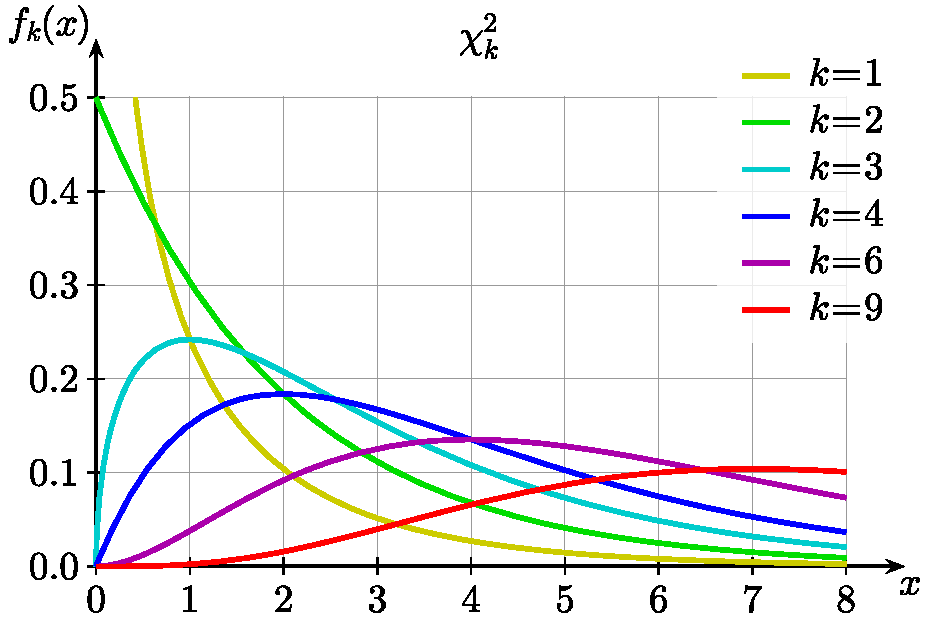
\includegraphics[width=0.7\textwidth]{../Diagrams/Chi-square.pdf}
  \caption{Illustration of how the \(\chi_{(\nu)}^2\) distribution looks with increasing degree of freedom \(\nu\).}
  \label{fig:chi-square}
\end{figure}
\begin{stbox}{General Information}
  \begin{itemize}
    \item Properties of chi-squared distributions.
    \begin{itemize}
      \item \(\E(X)=\nu\) and \(\Var(X)=2\nu\).
      % , and the mode of \(X\) is \(\max\{k-2,0\}\).
      \item The \(\chi_{(\nu)}^2\) distribution tends to a normal distribution as \(\nu\to\infty\).
      \item Suppose \(Z_i\sim\Normal(0,1)\) are independent. Then, \(Z_1^2+\dots+Z_n^2\sim\chi^2_{(n)}\).
      \item If \(X\sim\chi_{(\nu)}^2\) and \(Y\sim\chi_{(\upsilon)}^2\), then \(X+Y\sim\chi_{(\nu+\upsilon)}^2\).
    \end{itemize}
    \item A goodness-of-fit test.
    \begin{enumerate}
      \item Let [\(X\) in context].
      \item \emph{Note.} Use a pen to draw any necessary tables.

      \begin{tabular}{|ll|}
        \hline
        Test & \(H_0\colon\text{[\(X\) follows the distribution in context]}\)\\
        against &\(H_1\colon\text{[\(X\) does not follows the distribution in context]}\)\\
        \multicolumn{2}{|l|}{at the \(100\alpha\%\) significance level.}\\
        \hline
      \end{tabular}
      \item ~
      \begin{table}[H]
        \centering
        \begin{tabular}{|Sc|Sc|Sc|Sc|Sc|}
          \hline
          \(x\) & \(x_1\) & \(x_2\) & \(\cdots\) & \(x_n\)\\
          \hline
          \(f_i\) & \(f_1\) & \(f_2\) & \(\cdots\) & \(f_n\)\\
          \hline
          \(e_i\) & \(e_1\) & \(e_2\) & \(\cdots\) & \(e_n\)\\
          \hline
          \(\dfrac{(f_i-e_i)^2}{e_i}\) & \(\dfrac{(f_1-e_1)^2}{e_1}\) & \(\dfrac{(f_2-e_2)^2}{e_2}\) & \(\cdots\) & \(\dfrac{(f_n-e_n)^2}{e_n}\)\\
          \hline
        \end{tabular}
        \caption{Observed and expected frequencies for a goodness-of-fit test}
        \label{table:goodness-of-fit-test}
      \end{table}
      \item Check whether \(e_i\geq 5\) for each of the \(n\) classes. If it isn't, we need to combine \emph{just enough} adjacent classes, till they do. Working-wise, use some underbraces/overbraces to indicate the combined values. 
      \item Under \(H_0\), the test statistic is
      \[\chi^2=\sum_{i=1}^{n}{\frac{(F_i-E_i)^2}{E_i}}\sim\chi_{(\nu)}^2.\]
      Here, \(n\coloneq\#\text{classes}\) and \(\nu=(\#\text{classes}-\#\text{estimated parameters})-1\).
      \item Continue as per usual, calculating the critical region \(\chi_{(\nu)}^2>\chi^2_{(\nu,1-\alpha)}\) or the \(p\)-value.
    \end{enumerate}
  \end{itemize}
\end{stbox}
\begin{GCSkills}{}
  \begin{itemize}
    \item To find the value of \(\chi^2_{(\nu,1-\alpha)}\), which satisfies \(\Prob\left(X>\chi^2_{(\nu,1-\alpha)}\right)=\alpha\), we use the table in the \href{https://www.seab.gov.sg/docs/default-source/national-examinations/syllabus/alevel/2022syllabus/List_MF26_y22_sy.pdf}{MF26 formula sheet (Page 9)}. Unfortunately, there is no inverse \(\chi^2\) function available.
    \item For the \(p\)-value:
    \begin{center}
      \texttt{stat} \(\Longrightarrow\) \texttt{TESTS} \(\Longrightarrow\) \texttt{D:\(\chi^2\)GOF-Test\dots}
    \end{center}
  \end{itemize}
\end{GCSkills}
\begin{note}
  If \(X\) follows a \emph{discrete} uniform distribution, we must state it out in words. We cannot write \(X\sim\operatorname{U}(\mu,\sigma^2)\) as this would denote that \(X\) is a \emph{continuous} random variable. But if \(X\sim\Binom(n,p)\) (or \(X\sim\Poisson(\lambda)\), etc), then we can just denote it as such. 
\end{note}
\begin{example}{\(\#\text{estimated parameters}=0\)}{}
  Given \(X\sim\Normal(0,1)\) (note how the \emph{population parameters} that define the distribution are \emph{known}), the degree of freedom \(\nu=\#\text{estimated parameters}\eqcolon n\).
\end{example}
\begin{example}{\(\#\text{estimated parameters}=1\)}{}
  Consider when \(X\sim\Binom(m,p)\), such that the expected frequency for each of the \(n\) classes is at least 5, but we do not know the exact value of \(p\). So, we \emph{estimate} it according to the sample given. Then, the degree of freedom is \(\nu=n-1-1=n-2\).
\end{example}
\begin{example}{\(\#\text{estimated parameters}=2\)}{}
  Similarly, suppose \(X\sim\Normal(\mu,\sigma^2)\), such that the expected frequency of each of the \(n\) classes is at least 5, and the true values of \(\mu\) and \(\sigma^2\) are unknown. In this case, the degree of freedom \(\nu=n-2-1=n-3\). 
\end{example}
\begin{note}
  Consider when we are testing 
\begin{center}
    \begin{tabular}{|ll|}
      \hline
      Test & \(H_0\colon X\sim\Normal(\mu,\sigma^2)\)\\
      against &\(H_1\colon X\not\sim\Normal(\mu,\sigma^2)\)\\
      \multicolumn{2}{|l|}{at the \(100\alpha\%\) significance level.}\\
      \hline
    \end{tabular} 
\end{center}
So, we want to fill up the values of \(e_i\) below.
\begin{table}[H]
  \centering
  \begin{tabular}{|Sc|Sc|Sc|Sc|Sc|}
    \hline
    \(x\) & \(a_1\leq x_1\leq a_2\) & \(a_2\leq x_2\leq a_3\) & \(\cdots\) & \(a_n\leq x_n\leq a_{n+1}\)\\
    \hline
    \(f_i\) & \(f_1\) & \(f_2\) & \(\cdots\) & \(f_n\)\\
    \hline
    \(e_i\) & \cellcolor{yellow} \(e_1\) & \(e_2\) & \(\cdots\) & \cellcolor{yellow} \(e_n\)\\
    \hline
  \end{tabular}
  \caption{Observed and expected frequencies when testing goodness-of-fit with a normal distribution.}
  \label{table:gof-normal} 
\end{table}
Let the sample size \(\sum f_i\) be \(m\). Then, we should calculate \(e_1=m\Prob(\highlight[green!50]{-\infty}<X\leq a_2)\) and \(e_n=m\Prob(a_n\leq X<\highlight[green!50]{\infty})\), instead of \(e_1=m\Prob(\highlight[red!30]{a_1}\leq X\leq a_2)\) or \(e_n=m\Prob(a_n\leq X\leq\highlight[red!30]{a_{n+1}})\). Similarly, for goodness-of-fit tests with Poisson and Geometric distributions, we must also be careful in ensuring that we account for \emph{all} possible values which \(X\) can take on, in calculating \(e_i\).
\end{note}
\begin{note}
  Suppose we are given a question of the following form.

  \vspace{-0.5\baselineskip}\rule{20cm-137.0549pt}{0.05mm}

  Some context\dots 
  \begin{table}[H]
    \centering
    \begin{tabular}{|Sc|Sc|Sc|Sc|Sc|}
      \hline
      \(x_i\) & \(x_1\) & \(x_2\) & \(\cdots\) & \(x_n\)\\
      \hline
      \(f_i\) & \(f_1\) & \(f_2\) & \(\cdots\) & \(f_n\)\\
      \hline
    \end{tabular}
    \caption{Some data.}
    \label{table:some-chi-data}
  \end{table}
  \begin{enumerate}[label=(\roman*)]
    \item Show, at the \(100\alpha\)\% significance level, that the data does not support the hypothesis of \(X\sim\operatorname{Geo}(p)\) with \(p=0.5\).
    \item State how the test in (i) would have to be amended to test the hypothesis of a geometric distribution for an \emph{unspecified value of \(p\)}.
  \end{enumerate}

  \rule{20cm-137.0549pt}{0.05mm}
  Then, for (ii), two main changes have to be made:
  \begin{enumerate}
    \item Estimate the value of \(p\) by computing the sample mean \(\widebar{x}\) and letting \(p=1/\widebar{x}\).
    \item Adjust the degree of freedom from 4 to \(4-1=3\), as there is one more restriction, that the mean must agree.
  \end{enumerate}
  (The phrasing is similar for gof tests for other distributions; simply use the appropriate estimators for the unknown population parameters.)
\end{note}
\begin{stbox}{}
  Tests of independence. 
  \begin{enumerate}
    \item Let [\(X\) in context].
    \item 
    \begin{tabular}{|ll|}
      \hline
      Test & \(H_0\colon\text{[\(X\) in context] is independent of [\(Y\) in context]}\)\\
      against &\(H_1\colon\text{[\(X\) in context] is dependent on [\(Y\) in context]}\)\\
      \multicolumn{2}{|l|}{at the \(100\alpha\%\) significance level.}\\
      \hline
    \end{tabular}
    \item \emph{Note}. Unless the question asks for it, we do not need to write \(\left[ \frac{(f_i-e_i)^2}{e_i} \right]\) or its corresponding values, in the following table.
    \begin{table}[H]
      \hypertarget{table:tests-of-indepedence}{}
      \centering
      \begin{tabular}{ScSc|Sc|Sc|Sc|Sc|Sc}
        \cline{1-6}
        % &&\multicolumn{4}{Sc|}{\(X\)}&\\
        % \cline{3-7}
        % && \(x_1\) & \(x_2\) & \(\cdots\) & \(x_n\) & \multicolumn{1}{Sc|}{Total}\\
        \multicolumn{2}{|Sc|}{\multirow{2}{*}{\(f_i\) \((e_i)\) \(\left[ \frac{(f_i-e_i)^2}{e_i} \right]\)}} &\multicolumn{4}{Sc|}{\(X\)}&\\
        \cline{3-7}
        \multicolumn{2}{|Sc|}{}& \(x_1\) & \(x_2\) & \(\cdots\) & \(x_n\) & \multicolumn{1}{Sc|}{Total}\\
        \hline
        \multicolumn{1}{|Sc|}{\multirow{4}{*}{\(Y\)}}&\(y_1\)&&&&&\multicolumn{1}{Sc|}{\(t_{r_1}\)}\\ 
        \cline{2-7}
        \multicolumn{1}{|Sc|}{}&\(y_2\)&&&&&\multicolumn{1}{Sc|}{\(t_{r_2}\)}\\ 
        \cline{2-7}
        \multicolumn{1}{|Sc|}{}&\(\vdots\)&&&&&\multicolumn{1}{Sc|}{\vdots}\\
        \cline{2-7}
        \multicolumn{1}{|Sc|}{}&\(y_m\)&&&&&\multicolumn{1}{Sc|}{\(t_{r_m}\)}\\  
        \hline
        \multicolumn{1}{Sc|}{}& Total & \(t_{c_1}\) & \(t_{c_2}\) & \(\cdots\) & \(t_{c_n}\) & \multicolumn{1}{Sc|}{\(\sum{t_{r_i}}+\sum{t_{c_i}}\)}\\ 
        \cline{2-7}
      \end{tabular}
      \caption{\emph{Expected} frequencies for a test of independence.}
      \label{table:tests-of-indepedence}
    \end{table}
    \item Under \(H_0\), the test statistic is
    \[\chi^2=\sum_{i=1}^{n}{\frac{(F_i-E_i)^2}{E_i}}\sim\chi_{(\nu)}^2.\]
    Here, \(n\coloneq\#\text{cols}\) and \(\nu=(\#\text{rows}-1)(\#\text{cols}-1)\).
    \item Continue as per usual, calculating the critical region \(\chi_{(\nu)}^2>\chi^2_{(\nu,1-\alpha)}\) or the \(p\)-value.
  \end{enumerate}
\end{stbox}
\begin{GCSkills}{}
  Key in the matrix of \emph{\textcolor{green!70!black}{observed} frequencies} (not Table \hyperlink{table:tests-of-indepedence}{\textcolor{red}{1.2}} of \emph{\textcolor{red}{expected}} frequencies): 
  \begin{center}
    \texttt{2nd} \(\Longrightarrow\) \(\texttt{x}^{-1}\) \(\Longrightarrow\) \texttt{EDIT} \(\Longrightarrow\) \texttt{[A]}.
  \end{center}
  Then, conduct the test for independence:
  \begin{center}
    \texttt{stat} \(\Longrightarrow\) \texttt{TESTS} \(\Longrightarrow\) \texttt{C:\(\chi^2\)-Test\dots}
  \end{center}
\end{GCSkills}
\begin{note}
  If it's unclear as to what is to be stated as independent/dependent in the hypotheses, consider the expected values and how they relate to the context.  
\end{note}
\begin{example}{}{}
  \label{eg:infering-independence-relation}
  Consider the following context:
  \begin{table}[H]
    \centering
    \begin{tabular}{ScSc}
      \toprule
      Statement & \textcolor{green!70!black}{Independent}/\textcolor{red}{Dependent}?\\
      \midrule
      There is consistency in the marking of the two T.A.s. & ?\\
      There is no consistency in the marking of the two T.A.s. & ?\\
      \bottomrule  
    \end{tabular}
    \caption{Two statements on the relationship between the marks awarded and the T.A. marking.}
    % , which can be confusing to interpret
    \label{table:NOT-FILLED-infering-independence-relation-hypotheses}
  \end{table}
  Then, under \(H_0\) --- the independence claim --- the expected frequencies are as stated below.
  \begin{table}[H]
    \centering
    \begin{tabular}{ScScScScSc}
      \toprule  
      \multicolumn{2}{Sc}{\multirow{2}{*}{\(e_{ij}\)}} & \multicolumn{3}{Sc}{Grade}\\
      && \(A\) & \(B\) & \(C\)\\
      \midrule
      \multirow{2}{*}{\rotatebox[origin=c]{90}{T.A.}} & \(X\) & \(a\) & \(b\) & \(c\)\\
      & \(Y\) & \(a\) & \(b\) & \(c\)\\
      \bottomrule
    \end{tabular}
    \caption{Expected frequencies.}
    \label{table:infering-independence-relation-data}
  \end{table}
  Since \(e_{1j}=e_{2j}\) for all \(1\leq j\leq 3\), we infer the following.
  \begin{table}[H]
    \centering
    \begin{tabular}{ScSc}
      \toprule
      Statement & \textcolor{green!70!black}{Independent}/\textcolor{red}{Dependent}?\\
      \midrule
      There is consistency in the marking of the two T.A.s. & \textcolor{green!70!black}{Independent}\\
      There is no consistency in the marking of the two T.A.s. & \textcolor{red}{Dependent}\\
      \bottomrule  
    \end{tabular}
    \caption{Which statement corresponds to independence and which coresponds to dependence.}
    \label{table:FILLED-infering-independence-relation-hypotheses}
  \end{table}
\end{example}
\begin{note}
  If the question says to ``use an approximate \(\chi^2\)-statistic\dots'', then we must use the critical region method. It is incorrect to use the \(p\)-value.
\end{note}
\begin{note}
  Consider when we are asked to state which cells correspond to the highest contributions to the test statistic, and relate that back to the context of the question. Then:
  \begin{enumerate}
    \item State the cells in the form (\rule{0.5cm}{0.05mm},\ \rule{0.5cm}{0.05mm}). E.g. (High, Good) and (Low, Good).
    \item In table \ref{table:tests-of-indepedence}, add an asterisk to each of these cells. E.g. 
    \begin{tabular}{|Sc|}
      \hline
      1 \((5)\) \([10.1]^{*}\)\\
      \hline
    \end{tabular}\ .
    \item Use words that imply correlation and \emph{not} causation. E.g. directly associated, correlates with, etc.
  \end{enumerate}
\end{note}
\begin{note}
  On a similar note, if the question asks ``Can it can be concluded that\dots'', but is unclear about whether it's implying correlation or causation, it may be safer to explain both ways. i.e. what correlation is there and why is there no causation. 
\end{note}
\begin{note}
  Explain why we cannot conclude any casual relationships from a test of independence.
  \begin{center}
    \parbox{0.9\textwidth}{
      No, the above test does not reflect the actual casual relationship between the two factors, if it exists. Rather, it merely suggests that they are not independent.
    }
  \end{center}
\end{note}
\begin{note}
  Explain why we cannot apply a \(\chi^2\)-test for independence using the data given.
  \begin{center}
    \parbox{0.9\textwidth}{
      The expeceted frequency for (\rule{0.5cm}{0.05mm},\ \rule{0.5cm}{0.05mm}) is \(\rule{0.5cm}{0.05mm}<5\). If we combine the columns, the degree of freedom \(\nu=1\cdot 0=0\). If we combine the rows, \(\nu=0\cdot 1=0\). Thus, we cannot apply a \(\chi^2\)-test for independence. 
    }
  \end{center}
\end{note}

\chapter{Correlation and Linear Regression}
\begin{note}
  A good scatter diagram should follow the guidelines below.
  \begin{itemize}
    \item The relative position of each point on the scatter diagram should be clearly shown.
    \item The range of values for the set of data should be clearly shown by marking out the extreme \(x\) and \(y\) values on the corresponding axis.
    \item The axes should be labeled clearly with the variables.
  \end{itemize}
\end{note}
\begin{stbox}{General Information}
  \begin{itemize}
    \item The Product Moment Correlation Coefficient is a measure of the linear correlation between two variables. It is defined by
    \[r=\frac{\sum{(x-\widebar{x})(y-\widebar{y})}}{\sqrt{\sum{(x-\widebar{x})^2}\sum{(y-\widebar{y})^2}}}=\frac{\sum{xy}-\dfrac{\sum{x}\sum{y}}{n}}{\sqrt{\left[\sum{x^2}-\dfrac{\left(\sum{x}\right)^2}{n}\right]\left[\sum{y^2}-\dfrac{\left(\sum{y}\right)^2}{n}\right]}},\]
    which takes on a value from 0 to 1.
    \item When \(r=0\), there is no linear relationship. But, a nonlinear relationship may be present. Additionally, the regression lines are perpendicular.
    \item The closer the value of \(r\) is to 1 (or -1), the stronger the positive (or negative) linear correlation. Furthermore, the regression lines coincide.
    \begin{center}
      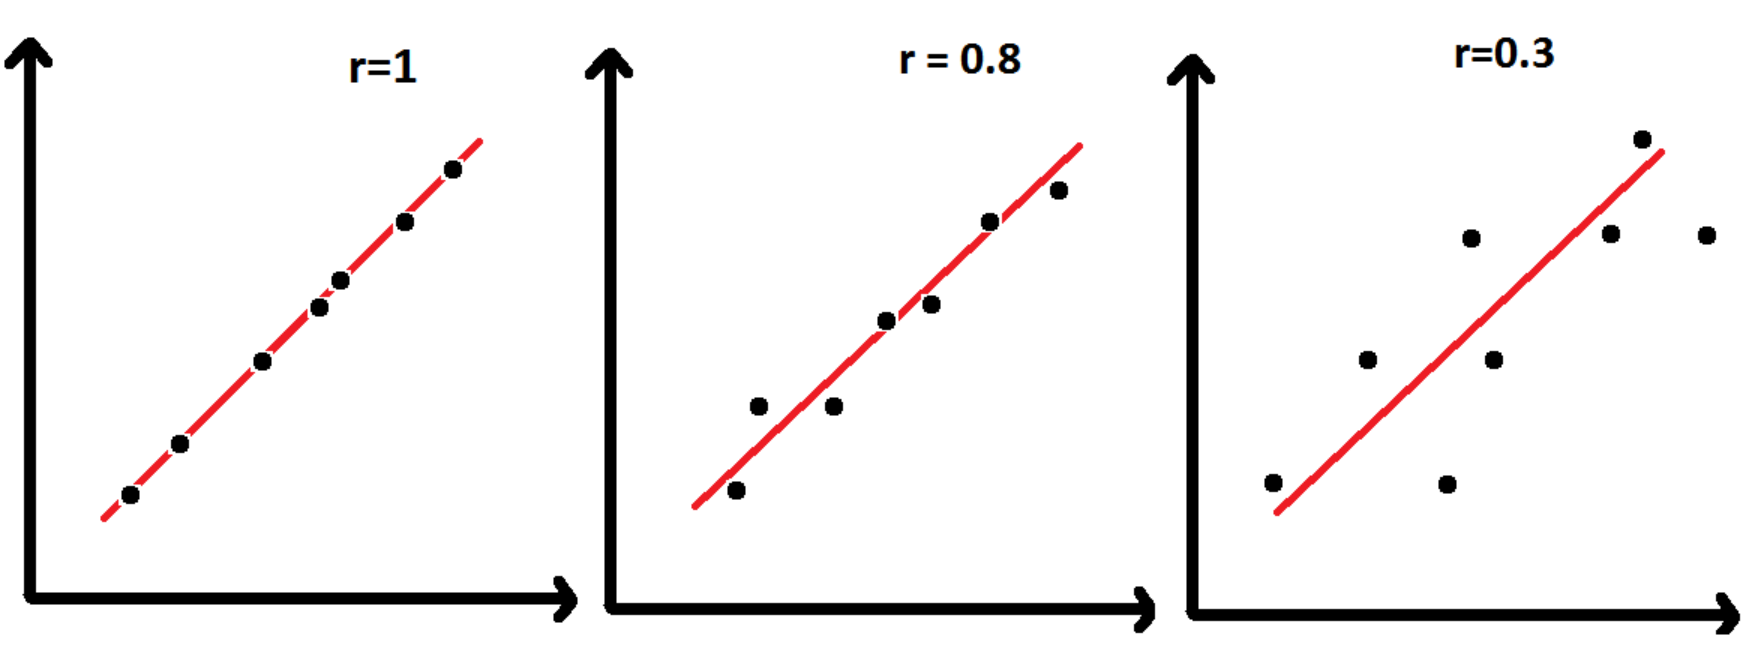
\includegraphics[scale=0.3]{../images/Product Moment Correlation Coefficient 1.png}
      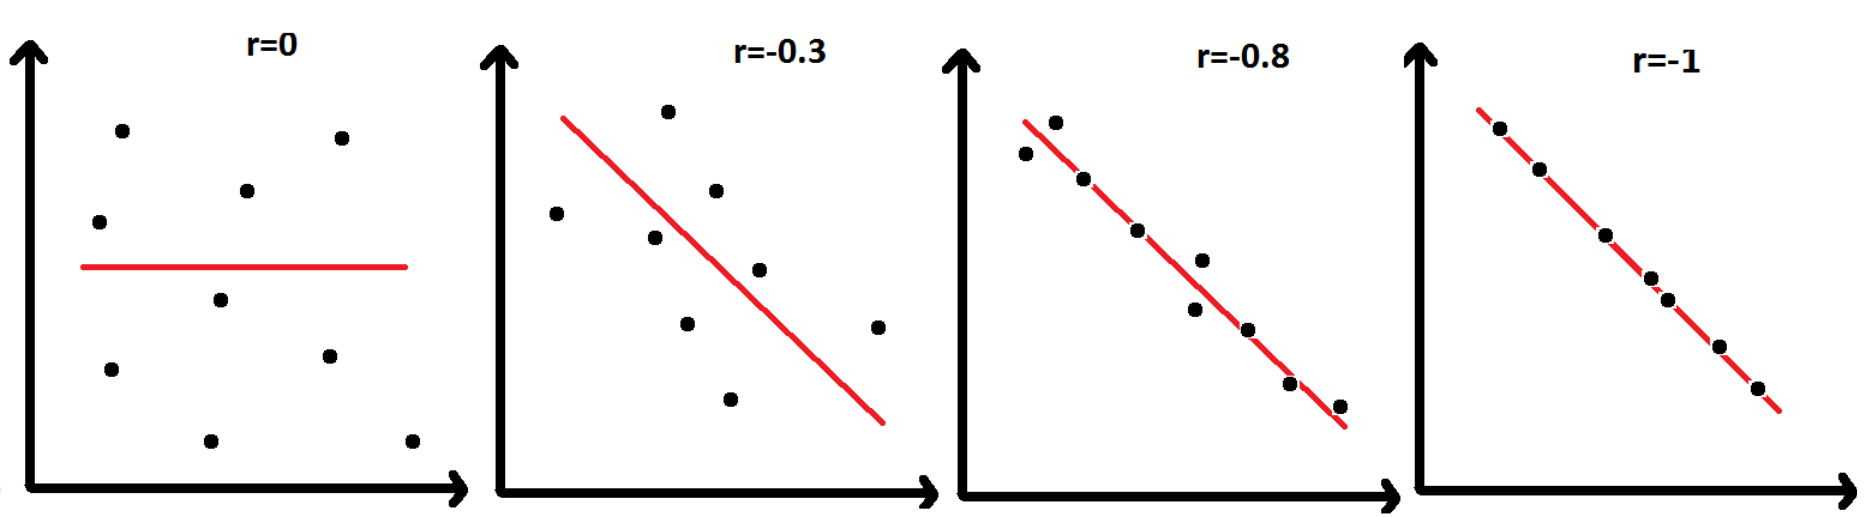
\includegraphics[scale=0.4]{../images/Product Moment Correlation Coefficient 2.png}
    \end{center}
    \item The regression line of \(y\) on \(x\) minimises the sum of squares deviation (error) in the \(y\)-direction. (i.e. we are assuming \(x\) is the independent variable whose values are known exactly.) It is given by
    \[y=\widebar{y}+b(x-\widebar{x}),\qquad\text{where}\qquad b=\frac{\sum{(x-\widebar{x})(y-\widebar{y})}}{\sum{(x-\widebar{x})^2}}=\frac{\sum{xy}-\dfrac{\sum{x}\sum{y}}{n}}{\sum{x^2}-\dfrac{\left(\sum{x}\right)^2}{n}}.\] 
    \item The regression lines of \(y\) on \(x\) and \(x\) on \(y\) intersect at \((\widebar{x},\widebar{y})\).
    \item Say we are given the value of one variable, and asked to approximate the the value of the other variable. Then, we should always use the line of the \emph{dependent} variable on the \emph{independent}.
    \item Estimations should not be taken for data outside the range of the sample provided, even if the value of \(r\) is close to 1.
  \end{itemize}
\end{stbox}

\chapter{Non-Parametric Tests}
\section{Sign tests}
\begin{stbox}{General Information}
  \begin{itemize}
    \item A \emph{sign test}.
    \begin{enumerate}
      \item Let \(m\) be the population median of \(D=\rule{1.5cm}{0.01mm}-\rule{1.5cm}{0.01mm}\).
      \item 
      \begin{tabular}{|ll|}
        \hline
        Test & \(H_0\colon m=m_0\)\\
        against &\(H_1\colon\) 
        \begin{enumerate*}[itemjoin={\quad}]
          \item \(m<m_0\),
          \item \(m\neq m_0\),\quad or
          \item \(m>m_0\),
        \end{enumerate*}\\
        \multicolumn{2}{|l|}{at the \(100\alpha\%\) significance level.}\\
        \hline
      \end{tabular}
      \item ~
      \begin{table}[H]
        \centering
        \begin{tabular}{|Sc|Sc|Sc|Sc|Sc|Sc|}
          \hline
          [label in context] & 1 & 2 & 3 & \(\cdots\) & \(n\)\\
          \hline 
          Sign & \(+\) & \(0\) & \(-\) & \(\cdots\) & \(+\)\\
          \hline
        \end{tabular}
        \caption{The signs of \(d_1,d_2,\dots,d_n\), for a sign test. Instead of \(1,2,\dots,n\) the labeling/column headers can differ in the given context. E.g. \(A,B,\dots,K\). Similarly, the signs here are mere examples; the \(i\)th sign cell should be filled with \(+\) (\(-\)) [0] if \(\operatorname{sgn}(d_i)=1\) (\(=-1\)) [\(=0\)].}
        \label{table:sign-test-working-table}
      \end{table}
      \item Let \(X_{+}\) be the number of \(`+'\). Under \(H_0\), \(X_{+}\sim\Binom(\hyperlink{non-parametric-tests-n-value}{n},1/2)\), \(x_{+}=11\). (Alternatively, \(X_{-}\) can also be used.)
      \item Since \(p\text{-value}=\rule{1cm}{0.01mm}<100\alpha\%\) (\(\geq 100\alpha\%\)), there is sufficient (insufficient) evidence, at the \(100\alpha\%\) significance level, to conclude that [\(H_1\) in context].
    \end{enumerate}
    \item \emph{Note.} The \(p\)-value for a sign test is given by
    \begin{table}[H]
      \centering
      \begin{tabular}{ScScScSc}
        \toprule
        \(H_1\) & \(m<m_0\) & \(m>m_0\) & \(m\neq m_0\)\\
        \midrule
        \(X_{+}\) & \(\Prob(X_{+}\leq x_{+})\) & \(\Prob(X_{+}\geq x_{+})\) & \(2\min\{\Prob(X_{+}\geq x_{+}),\Prob(X_{+})\leq x_{+}\}\)\\
        \midrule
        \(X_{-}\) & \(\Prob(X_{-}\geq x_{-})\) & \(\Prob(X_{-}\leq x_{-})\) & \(2\min\{\Prob(X_{-}\geq x_{-}),\Prob(X_{-})\leq x_{-}\}\)\\
        \bottomrule
      \end{tabular}
      \caption{The \(p\)-value for a sign test.}
      \label{table:sign-test-p-value}
    \end{table}
  \end{itemize}
\end{stbox}
\begin{note}
  Sign test. Suppose we have \(H_1\colon m\neq m_0\). To find the range of values of \(x_{+}\) that result in the rejection of \(H_0\), use GC to compute the following tables.
  \begin{table}[H]
    \centering
    \begin{tabular}{|Sc|Sc|}
      \hline
      \(x_{+}\) & \(\alpha/2-2\Prob(X_{+}\leq x_{+})\)\\
      \hline
      \(n-1\) & \(\rule{0.5cm}{0.01mm}>0\)\\
      \hline
      \(n\) & \(\rule{0.5cm}{0.01mm}>0\)\\
      \hline
      \(n+1\) & \(\rule{0.5cm}{0.01mm}<0\)\\
      \hline
    \end{tabular}\hspace{1cm}
    \begin{tabular}{|Sc|Sc|}
      \hline
      \(x_{+}\) & \(\alpha/2-2\Prob(X_{+}\geq x_{+})\)\\
      \hline
      \(m-1\) & \(\rule{0.5cm}{0.01mm}<0\)\\
      \hline
      \(m\) & \(\rule{0.5cm}{0.01mm}<0\)\\
      \hline
      \(m+1\) & \(\rule{0.5cm}{0.01mm}>0\)\\
      \hline
    \end{tabular} 
  \end{table}
  Then, we conclude that \(x_{+}\leq n\) or \(x_{+}\geq m\).
\end{note}
\section{Wilcoxon matched-pairs signed rank tests}
\begin{stbox}{General Information}
  \begin{itemize}
    \item A Wilcoxon matched-pairs signed rank test. 
    \begin{enumerate}
      \item Let \(m\) be the population median of \(D=\rule{1.5cm}{0.01mm}-\rule{1.5cm}{0.01mm}\).
      \item 
      \begin{tabular}{|ll|}
        \hline
        Test & \(H_0\colon m=0\)\\
        against &\(H_1\colon\) 
        \begin{enumerate*}[itemjoin={\quad}]
          \item \(m<\highlight[yellow]{0}\),
          \item \(m\neq \highlight[yellow]{0}\),\quad or
          \item \(m>\highlight[yellow]{0}\),
        \end{enumerate*}\\
        \multicolumn{2}{|l|}{at the \(100\alpha\%\) significance level.}\\
        \hline
      \end{tabular}
      \item ~
      \begin{table}[H]
        \centering
        \begin{tabular}{|Sc|Sc|Sc|Sc|Sc|Sc|}
          \hline
          [label in context] & 1 & 2 & 3 & \(\cdots\) & \(n\)\\
          \hline 
          \(D\) & \(d_1\) & \(0\) & \(d_3\) & \(\cdots\) & \(d_n\)\\
          \hline
          Rank & \(1\) &  & \(5\) & \(\cdots\) & \(2\)\\
          \hline
        \end{tabular}
        \caption{The value of the differences \(d_1,d_2,\dots,d_n\), which are then ranked according to their absolute size \(\lvert d_i \rvert\). If \(d_i=0\), simply leave the corresponding cell, for rank, blank.}
        \label{table:wilcoxon-working-table}
      \end{table}
      \item
      \begin{itemize}[label=\(\circ\)]
        \item \(t_{-}=\rule{0.5cm}{0.01mm}+\rule{0.5cm}{0.01mm}+\dots+\rule{0.5cm}{0.01mm}=\rule{0.5cm}{0.01mm}\)
        \item \(t_{+}=\rule{0.5cm}{0.01mm}+\rule{0.5cm}{0.01mm}+\dots+\rule{0.5cm}{0.01mm}=\rule{0.5cm}{0.01mm}\)
        \item The test statistic is \(T\coloneq\min\{T_{-},T_{+}\}=\rule{0.5cm}{0.01mm}\).
        \item Reject \(H_0\) if \(T=\rule{0.5cm}{0.01mm}\). (see table \ref{table:wilcoxon-critical-region})
      \end{itemize}
      \item Since \(t=\rule{0.5cm}{0.01mm}\,\square\, \rule{0.5cm}{0.01mm}\), there is sufficient/insufficient evidence, at the \(100\alpha\%\) significance level, to conclude that [\(H_1\) in context].
    \end{enumerate}
    \item The test statistics \(T_{+}\) and \(T_{-}\) can also be used, depending on our preference.
      \item The critical regions for a Wilcoxon test, for each alternative hypothesis and test statistic \(T_{-}\) or \(T_{+}\). The value of \(c\) is obtained from MF26\(^{\hyperlink{non-parametric-tests-n-value}{*}}\). 
      
      \emph{Note.} the value of \(c\) may differ for a one-tail vs a two-tail test, so look at the table carefully, to obtain the correct value.
      \begin{table}[H]
        \centering
        \setlength{\tabcolsep}{12pt}
        \begin{tabular}{ScScScSc}
          \toprule
          \(H_1\) & \(m<m_0\) & \(m>m_0\) & \(m\neq m_0\)\\
          \midrule
          \(T_{+}\) & \(T_{+}\leq c\) & \(T_{+}\geq \dfrac{n(n+1)}{2}-c\) & \(T_{+}\leq c\)\quad or\quad\(T_{+}\geq \dfrac{n(n+1)}{2}-c\)\\
          \midrule
          \(T_{-}\) & \(T_{-}\geq \dfrac{n(n+1)}{2}-c\) & \(T_{-}\leq c\) & \(T_{-}\leq c\)\quad or\quad\(T_{-}\geq \dfrac{n(n+1)}{2}-c\)\\
          \midrule
          \(T\) & \multicolumn{2}{Sc}{\(T\leq c^{\hyperlink{wilcoxson-T=min-note}{1}}\)} & \(T\leq c\)\quad or\quad\(T\geq \dfrac{n(n+1)}{2}-c\)\\
          \bottomrule
        \end{tabular}
        \caption{The critical regions for Wilcoxon tests.}
        \label{table:wilcoxon-critical-region}
      \end{table}
      \begin{footnotesize}
        {}\(^{\protect\hypertarget{wilcoxson-T=min-note}{1}}\)Assuming \(T_{-}\geq T_{+}\) for \(m<m_0\), and \(T_{+}\geq T_{-}\) for \(m>m_0\).
      \end{footnotesize}
      \setlength{\tabcolsep}{6pt}
      \item For large sample sizes \(n\geq 21\), we use the approximation 
      \[T\sim\Normal\left( \frac{n(n+1)}{4},\frac{n(n+1)(2n+1)}{24} \right)\]
      and conduct a one/two-tailed \(z\)-test.
  \end{itemize}
\end{stbox}
\begin{note}\hypertarget{non-parametric-tests-n-value}{}
  The value of \(n\) in both tests should be the total number of columns minus the number of columns with \(d=0\). i.e.
  \[n\coloneq\#\text{cols}-\#\{i \,\vert\, d_i\neq 0\}.\]
\end{note}
\begin{note}
  If we need to use both the sign test and a Wilcoxon test on the same sample, then consider creating just a single table, as shown below. 
  \begin{table}[H]
    \centering
    \begin{tabular}{|Sc|Sc|Sc|Sc|Sc|Sc|}
      \hline
      [label in context] & 1 & 2 & 3 & \(\cdots\) & \(n\)\\
      \hline 
      \(D\) & \(d_1\) & \(0\) & \(d_3\) & \(\cdots\) & \(d_n\)\\
      \hline
      Sign & \(+\) & \(0\) & \(-\) & \(\cdots\) & \(+\)\\
      \hline
      Rank & \(1\) &  & \(5\) & \(\cdots\) & \(2\)\\
      \hline
    \end{tabular}
    \caption{Combined table for both the sign test and Wilcoxon test.}
    \label{table:sign-Wilcoxon-combined}
  \end{table}
\end{note}
\begin{note}
  How do you improve the Wilcoxon test used in [the previous part]?
  \begin{center}
    Increase the sample size for the test.
  \end{center}
\end{note}
\begin{note}
  State the circumstances under which a non-parametric test would be used rather than a parametric test.
  \begin{center}
    \parbox{0.9\textwidth}{
      We use a non-parametric test, rather than a parametric test, when:
      \begin{enumerate}
        \item The population is not known to be normally distributed.
        \item The population mean is not the best way to measure tendency.
        \item The measurement scale has no predetermined rank or ordering. 
      \end{enumerate}
    }
  \end{center}
\end{note}
\begin{note}
  Why is it not appropriate to use a paired-sample \(t\)-test? 
  \begin{center}
    \parbox{0.9\textwidth}{
      There is no contextual evidence to support the assumption that \(D_1,D_2,\dots,D_n\) are normally distributed. So, conducting a paired-sample \(t\)-test may result in unreliable results, given our small sample size \(n\). 
    }
  \end{center}
\end{note}
\begin{note}
  State the precautions that should be taken to avoid (statistical) bias. 
  \begin{center}
    \parbox{0.9\textwidth}{
      Choose any approperate ones.
      \begin{enumerate}
        \item The test should be \emph{`blind'}. [Testers in context] should not know which of the [two variations involved in the test, in context] they are [tasting/wearing/etc, in context]. If the [testers] knew, their preconceptions may affect \rule{2cm}{0.01mm}.
        \item Pick a random sample of \(n\) [testers].
        \item The \emph{order} of the test --- whether the [first variation] or [second variation] comes first --- should be randomised.
        \item The [testers] should not communicate with each other.
        \item There should be sufficient rest time between the two runs, so that the running timing of the second run would not be affected due to fatigue.
      \end{enumerate}
    }
  \end{center}
\end{note}
\begin{note}
  Explain why it is better to conduct a \textcolor{green!70!black}{Wilcoxon} test than a \textcolor{red}{sign} test.
  \begin{center}
    \parbox{0.9\textwidth}{
     While a sign test only considers the sign of the differences, a Wilcoxon test takes into account both the sign and \emph{magnitude} of the differences. Therefore, a Wilcoxon test is more reliable, as it incorporates more information about the data.
    }
  \end{center}
  % \begin{center}
  %   \parbox{0.9\textwidth}{
      
  %   }
  % \end{center}
\end{note}
% \begin{note}
%   Explain why it might be better to conduct a sign test, rather than a Wilcoxon test. 
%   \begin{center}
%     \parbox{0.9\textwidth}{
      
%     }
%   \end{center}
% \end{note}
\begin{note}
  Explain why a sign test is more suitable/a \textcolor{red}{Wilcoxon} test is inappropriate.
  \begin{center}
    \parbox{0.9\textwidth}{
      Choose any approperiate ones
      \begin{enumerate}
        \item The data here is non-numeric and is not meausred on an ordinal scale. Hence, it is inapproperiate to conduct a Wilcoxon test. A sign test is better, as the data can still be represented by positie and negative responses --- denoting \rule{1cm}{0.01mm} and \rule{1cm}{0.01mm}, respectively.
        \item The magnitude of the differences is irrelevant because \rule{1cm}{0.01mm}. So, a sign test --- which only accounts for the sign of the differences --- is more appropriate.
        \item In this case, the data has too many \emph{tied ranks}. Thus, the conclusion obtained from a Wilcoxon test may not be reliable.
        \item An additional assumption that the differences \(D\) of \rule{1cm}{0.01mm} must be symmetric about the median. 
      \end{enumerate}
    }
  \end{center}
\end{note}
\begin{example}{A tricker question, involving an unknown in the data provided.}{}
  Let \(m\) be the median of \(D\colon X-Y\). For the data in Table \ref{table:wilcoxon-unknown-variable-raw-data}, assume that there are no tied ranks, and \(x_i\neq y_i\) for each \(1\leq i<j\leq 7\). Carry out a Wilcoxon test, at the \(5\%\) significance level, to determine if the data supports the alternative hypothesis \(H_1\colon m>0\).
  \begin{table}[H]
    \centering
    \begin{tabular}{ScScScScScScScSc}
      \toprule
      Index & \(1\) & \(2\) & \(3\) & \(4\) & \(5\) & \(6\) & \(7\)\\
      \midrule
      \(x_i\) & \(4\) & \(8\) & \(7\) & \(7\) & \(1\) & \(9\) & \(9\)\\
      \(y_i\) & \(6\) & \(9\) & \(3\) & \(4\) & \(a\) & \(1\) & \(2\)\\
      \bottomrule
    \end{tabular}
    \caption{Data with an unknown variable \(a\in {\mathbb{Z}^{+}}\).}
    \label{table:wilcoxon-unknown-variable-raw-data}
  \end{table}
  \rule{20cm-137.0549pt}{0.05mm}
  First, we calculate the differences. Since \(x_i\neq y_i\), we have \(a\neq 1\). In fact, \(a\neq 1,2,3,4,7,8\) because \(d_i\neq d_j\), for \(i\neq j\). Thus, \(a=6,7\) or \(a\geq 10\). The corresponding rank \(r_5\) is hence \(5\) or \(7\). 
  \begin{table}[H]
    \centering
    \begin{tabular}{Sc>{\columncolor[gray]{0.8}}Sc>{\columncolor[gray]{0.8}}ScScSc>{\columncolor[gray]{0.8}}ScScSc}
      \toprule
      Index & \(1\) & \(2\) & \(3\) & \(4\) & \(5\) & \(6\) & \(7\)\\
      \midrule
      \(d_i\) & \(-2\) & \(-1\) & \(4\) & \(3\) & \(1-a\) & \(8\) & \(7\)\\
      \(\lvert d_i \rvert\) & \(2\) & \(1\) & \(4\) & \(3\) & \(a-1\) & \(8\) & \(7\)\\
      rank \(r_i\) & \(2\) & \(1\) & \(4\) & \(3\) & \(r_5\) & \(r_6\) & \(r_7\)\\
      \bottomrule
    \end{tabular}
    \caption{The values of the differences \(d_i\) and the associated ranks. The columns highlighted in grey are those with negative differences \(d_i\).}
    \label{table:wilcoxon-unknown-variable-proceessed-data-with-calculated-differences}
  \end{table}
  Now,
  \[t_{-}=2+1+r_5=8,10 \qquad\text{and}\qquad t_{+}=7(7+1)/2-t_{-}=25-r_5=20,18.\]
  Hence, the test statistic \(T\coloneq\min\{T_{-},T_{+}\}=T_{-}\), where we reject \(H_0\) if \(T\leq 3\). So, since \(t_{-}=3+r_5>3\), we do not reject \(H_0\). 
\end{example}
\end{document}